% chapters/mathbg.tex
%  Second chapter in mathbg.tex

\section{Hamilton Jacobi Equations}
A Hamilton Jacobi equation (HJE) is a non-linear Partial Differential Equation of the form
\begin{eqnarray}
  H(\mathbf{x},u(\mathbf{x}),Du(\mathbf{x})) &=& 0 \;\; \text{in} \;\; \Omega \label{eq:1}\\
  u(\mathbf{x}) &=& \varphi(\mathbf{x}) \;\; \text{on} \;\; \partial \Omega \label{eq:2}
\end{eqnarray}
where $\mathbf{x} = (x_1,\dots,x_n) \in \mathbb{R}^n$, $u(\mathbf{x}) \in \mathbb{R}$ and $Du(\mathbf{x})$ is the first order derivative of u in $\mathbb{R}^n$, defined by,
\begin{equation}
  Du(\mathbf{x}) = \left(\frac{\partial u}{\partial x_1},\dots ,\frac{\partial u}{\partial x_n}\right)^T
\end{equation}

\noindent
The function $H(\mathbf{x},u(\mathbf{x}),Du(\mathbf{x})) : \Omega \times \mathbb{R} \times \mathbb{R}^n \to \mathbb{R}$ is known as the Hamiltonian. $u(\mathbf{x})$ is our unknown function. The problem defined by (\ref{eq:1})-(\ref{eq:2}) is known as the Dirichlet Boundary Value Problem (BVP). The other class of problem, known as the Cauchy Problem is given by,
\begin{eqnarray}
  \frac{\partial u }{\partial t} + H(\mathbf{x},t,u(\mathbf{x},t),Du(\mathbf{x},t)) &=& 0 \qquad \qquad \; \text{in} \;\; \Omega \times ]0,T] \label{eq:3}\\
  u(\mathbf{x},t) &=& \varphi(\mathbf{x},t) \qquad \text{on} \;\; \partial \Omega \times ]0,T]\label{eq:4}\\
  u(\mathbf{x},0) &=& u_0(\mathbf{x}) \qquad \;\; \text{in} \;\; \Omega
\end{eqnarray}

\noindent
The function $u_0(\mathbf{x})$ is known as the initial condition. These types of PDEs were investigated by the Irish Mathematician William Rowan Hamilton\cite{ham1,ham2}.

\section{Well Posedness}
According to Hadamard\cite{hadamard}, a mathematical model has to be well posed. A well posed problem has the following properties,
\begin{enumerate}
\item
\textbf{Existence} - There exists a solution to the problem.
\item
\textbf{Uniqueness} - There exists atmost one solution to the problem.
\item
\textbf{Stability} - The solution depends continuously on the data.
\end{enumerate}

\noindent
The existence of a solution to the HJE can be assured if we enlarge the space of functions under consideration. For example, as we will see soon enough, the Eikonal Equation has a solution in $C^0$, the space of continuous functions, but not in $C^1$, the space of continuously differentiable functions. The uniqueness of a problem is normally obtained by supplying additional information like initial/boundary data, so that we can capture the physically relevant solution. Stability is an important criterion while constructing the numerical schemes, as a small perturbation in the initial data should produce small changes in the solution to the PDE. This situation becomes relevant when we tend the mesh size $h \to 0$, the computed solution should converge to the exact solution of the PDE\cite{lax}.

\section{Viscosity Solutions}
\subsection{Need for Viscosity Solutions}
The Hamilton Jacobi Equations are normally not well-posed under the classical solution approach. The properties of existence and uniqueness in the classical sense are no longer satisfied.\\

\noindent
For example, when we consider solving the Eikonal Equation in 1D,
\begin{eqnarray}
  \lvert u' \rvert &=& 1 \qquad \text{in} \;\;\; \Omega \equiv (0,1)\label{eq:5}\\
  u &=& 0 \qquad \text{on} \;\;\; \partial \Omega \equiv \{0,1\}\label{eq:6}
\end{eqnarray}
which is a HJE, it can be shown that the solution to the problem does not exist in $C^1$. This can be easily proved using contradiction. Consider that we are looking for a solution $u \in C^1$. As we have, $u(0) = u(1) = 0$, by Rolle's Theorem, $\exists x_0 \in (0,1)$ such that $u'(x_0) = 0$, which contradicts (\ref{eq:5}). So $u \notin C^1$. This shows that, we have solutions that are not differentiable at certain points on the domain but $u \in C^0$. Such solutions satisfy the PDE in a ``weaker" sense and hence are called \textbf{weak solutions}.\\

\noindent
One can see that $u^+(x) = \frac{1}{2} - \left\lvert \frac{1}{2} - x\right\rvert$ is a \textit{weak} solution to the Dirichlet Problem (\ref{eq:5})-(\ref{eq:6}). But we can see that $u^-(x) = -u^+(x)$ is a solution to the problem as well. Hence, the classical approach becomes insufficient to guarantee a unique solution to the Dirichlet Problem.\\

\noindent
\subsection{Viscosity Solutions}
P.L.Lions and M.G.Crandall\cite{lions} came up with a setting to obtain the
existence and uniqueness properties for the Hamilton Jacobi
Equation. They are known as \textbf{viscosity solutions}. The term
\textbf{viscosity} is used because solution to the HJE is obtained by
adding a viscosity term $\epsilon u_{xx}$ to the HJE and letting
$\epsilon \to 0$ to obtain the solution to our original PDE. Before we
see how to obtain the viscosity solutions, we must find a way to deal
with the non-differentiable points in $C^0$ solutions. For this we
define \textbf{super differentials} and \textbf{sub
  differentials}. Super- and sub-differentials replaces the classical
derivatives at non-differentiable points in the functions and are
equivalent to the classical definition at differentiable points.

\noindent
For the following HJE,
\begin{eqnarray}
  H(\mathbf{x},\nabla u(\mathbf{x})) &=& 0 \qquad \text{in} \;\;\; \Omega\\
  u(\mathbf{x}) &=& \varphi(\mathbf{x}) \qquad \text{on} \;\;\; \partial \Omega
\end{eqnarray}
\begin{definition}
  A continuous function $u\in C^0$ is a viscosity solution to the HJE,
  if it satisfies the following conditions
  \begin{enumerate}
  \item \textbf{Viscosity Subsolution} : For any test function
    $\varphi \in C^1$, if $\mathbf{x_o}$ is the local maximum of
    $u-\varphi$, then
    \begin{equation}\nonumber
      H(\mathbf{x_o}, \nabla u(\mathbf{x_o}) ) \le 0
    \end{equation}

  \item \textbf{Viscosity Supersolution} : For any test function
    $\varphi \in C^1$, if $\mathbf{x_o}$ is the local minimum of
    $u-\varphi$, then
    \begin{equation}\nonumber
      H(\mathbf{x_o}, \nabla u(\mathbf{x_o}) ) \ge 0
    \end{equation}
  \end{enumerate}
  \label{def:1}
\end{definition}
An alternate, but an equivalent definition of the same is given using
sub- and super- differentials.
\begin{definition}
  A continuous function $u\in C^0$ is a viscosity solution to the HJE,
  if it satisfies the following conditions
  \begin{enumerate}
  \item \textbf{Viscosity Subsolution} : $H(\mathbf{x},p) \le 0$ for
    all $\mathbf{x} \in \mathbb{R}^n$ and $p\in D^+u$

  \item \textbf{Viscosity Supersolution} : $H(\mathbf{x},q) \ge 0$ for
    all $\mathbf{x} \in \mathbb{R}^n$ and $q\in D^-u$
  \end{enumerate}
  \label{def:2}
  where,
  \begin{eqnarray}
    D^+u &=& \left\{p \in \mathbb{R}^n \;\; \Big |\;\; \limsup\limits_{y\to x} \frac{u(y)-u(x) - p.(y-x)}{\lvert y-x \rvert} \le 0\right\}\label{eq:7}\\
    D^-u &=& \left\{q \in \mathbb{R}^n \;\; \Big |\;\; \liminf\limits_{y\to x} \frac{u(y)-u(x) - q.(y-x)}{\lvert y-x \rvert} \ge 0\right\}\label{eq:8}
  \end{eqnarray}
\end{definition}

\noindent
The sets $D^+u$ and $D^-u$ are known as the super- and
sub-differentials, respectively. A collection of some properties of
sub- and super-differentials are listed below. Refer \cite{yong} for more
details.
\begin{enumerate}
\item $D^+u$ and $D^-u$ are convex subsets of $\mathbb{R}^n$.
\item If $u$ is differentiable at any point $\mathbf{x}$, then
  \begin{equation}\nonumber
    \{Du(\mathbf{x})\} = D^+u(\mathbf{x}) = D^-u(\mathbf{x})
  \end{equation}
\item If for some $\mathbf{x}$, both $D^+u$ and $D^-u$ are non-empty,
  \begin{equation}\nonumber
    \{Du(\mathbf{x})\} = D^+u(\mathbf{x}) = D^-u(\mathbf{x})
  \end{equation}
\item
  $D^+(\alpha u)(\mathbf{x}) = \alpha D^+u(\mathbf{x}), \quad \alpha >
  0$
\item
  $D^+(\alpha u)(\mathbf{x}) = \alpha D^-u(\mathbf{x}), \quad \alpha <
  0$
\item
  $D^+(u+\varphi)(\mathbf{x}) = D^+u(\mathbf{x}) +
  D\varphi(\mathbf{x}), \quad \text{if} \;\varphi \in C^1$
\item
  $D^+u_\alpha(\mathbf{x}) = \alpha D^+u(\mathbf{x}) +
  (1-\alpha)D\varphi\nonumber$ \hspace{5mm} \text{where,}
  $\quad u_\alpha = \alpha u(\mathbf{x}) +
  (1-\alpha)\varphi(\mathbf{x)}\nonumber$
\end{enumerate}

\noindent
The following example illustrates the procedure for calculating the
super and sub-differentials of a function in 1D. We do this for
$u^+(x) = 1 - \lvert x \rvert$ and use them to isolate the viscosity
solution of the following Eikonal equation with Dirichlet boundary
data. (In fact we show that $u^+(x)$ is the viscosity solution to our
Dirichlet BVP).
\begin{eqnarray}
  |u'| &=& 1 \qquad \text{in} \;\; \Omega \equiv (-1,1)\\
  u &=& 0 \qquad \text {on} \;\; \partial \Omega \equiv \{-1,1\}
\end{eqnarray}
\begin{example}
  Super and sub differential of $u(x) = 1-\lvert x \rvert$\\

  \noindent
  \textbf{Super Differential} $D^+u$:\\

  \noindent
  We consider the case only when $x=0$, as $x=0$ is the only
  non-differentiable point. The classical definition of the derivative
  holds for the case $x\ne 0$ as the function is differentiable at
  these points. For full details, refer \cite{yong}
  \begin{enumerate}
  \item $x = 0$
    \begin{itemize}
    \item
      $y \ge 0 \implies \lvert y \rvert = y \implies 1 - \lvert y
      \rvert = 1 - y$
      \begin{eqnarray}
        &\iff&\limsup \limits_{y \to x} \frac{u(y)-u(x) - p(y-x)}{\lvert y -x \rvert} \le 0\\
        &\iff& \limsup \limits_{y \to 0} \frac{(1-y)-1 - p(y-0)}{\lvert y -0 \rvert} \le 0\\
        &\iff& \limsup \limits_{y \to 0} \frac{-y - py}{ y } \le 0\\
        \text{As} \quad y \ge 0 &\iff& -y-py \le 0 \implies y(1+p) \ge 0 \nonumber
                                       \implies p \ge -1
      \end{eqnarray}

    \item
      $y \le 0 \implies \lvert y \rvert = -y \implies 1 - \lvert y
      \rvert = 1 + y$
      \begin{eqnarray}
        &\iff&\limsup \limits_{y \to x} \frac{u(y)-u(x) - p(y-x)}{\lvert y -x \rvert} \le 0\\
        &\iff& \limsup \limits_{y \to 0} \frac{(1+y)-1 - p(y-0)}{\lvert y -0 \rvert} \le 0\\
        &\iff& \limsup \limits_{y \to 0} \frac{y - py}{ -y } \le 0\\
        \text{As} \quad -y \ge 0 &\iff& y-py \le 0 \implies y(1-p) \le 0 \nonumber
                                        \implies p \le 1
      \end{eqnarray}
    \end{itemize}
    From the two cases, we conclude that when $x=0$, $p\in[-1,1]$

  \item $x < 0$, we have from the classical definition $p = \{1\}$

  \item $x > 0$, we have from the classical definition $p = \{-1\}$
  \end{enumerate}
  Hence from the above steps, we conclude that the super differential
  of $1-\lvert x \rvert$ is
  \begin{eqnarray}
    D^+u = \left\{
    \begin{array}{ll}
      1 & x \le 0\\
      \left[-1,1\right] & x = 0\\
      -1 & x\ge 0
    \end{array}
           \right.\label{eq:9}
  \end{eqnarray}

\noindent
Following the same procedure, we can find the sub-differential of $1-\lvert x \rvert$.\\

\noindent
\textbf{Sub Differential} $D^-u$
\begin{enumerate}
\item $x = 0$
  \begin{itemize}
  \item
    $y \ge 0 \implies \lvert y \rvert = y \implies 1 - \lvert y \rvert
    = 1 - y$
    \begin{eqnarray}
      &\iff&\liminf \limits_{y \to x} \frac{u(y)-u(x) - p(y-x)}{\lvert y -x \rvert} \ge 0\\
      &\iff& \liminf\limits_{y \to 0} \frac{(1-y)-1 - p(y-0)}{\lvert y -0 \rvert} \ge 0\\
      &\iff& \liminf \limits_{y \to 0} \frac{-y - py}{ y } \ge 0\\
      \text{As} \quad y \ge 0 &\iff& -y-py \ge 0 \implies y(1+p) \le 0 \nonumber
                                     \implies p \le -1
    \end{eqnarray}

  \item
    $y \le 0 \implies \lvert y \rvert = -y \implies 1 - \lvert y
    \rvert = 1 + y$
    \begin{eqnarray}
      &\iff&\liminf \limits_{y \to x} \frac{u(y)-u(x) - p(y-x)}{\lvert y -x \rvert} \ge 0\\
      &\iff& \liminf \limits_{y \to 0} \frac{(1+y)-1 - p(y-0)}{\lvert y -0 \rvert} \ge 0\\
      &\iff& \liminf \limits_{y \to 0} \frac{y - py}{ -y } \ge 0\\
      \text{As} \quad -y \ge 0 &\iff& y-py \ge 0 \implies y(1-p) \ge 0 \nonumber
                                      \implies p \ge 1
    \end{eqnarray}
  \end{itemize}
  From the two cases, we conclude that when $x=0$, $p = \phi$

\item $x < 0$, we have from the classical definition $p = \{1\}$

\item $x > 0$, we have from the classical definition $p = \{-1\}$
\end{enumerate}
Hence from the above steps, we conclude that the sub differential of
$1-\lvert x \rvert$ is
\begin{eqnarray}
  D^-u = \left\{
  \begin{array}{ll}
    1 & x \le 0\\
    \emptyset & x = 0\\
    -1 & x\ge 0
  \end{array}
         \right. \label{eq:10}
\end{eqnarray}
\end{example}

\noindent
With the super- and sub- differentials in our hand, we now see how
this can be used to pick out the unique viscosity solution of the
Eikonal equation. Let us consider $u(x) = 1-\vert x \rvert$ and the
convex Hamiltonian $H(x,p) = \lvert p \rvert - 1$ for the Eikonal
equation. Now we have from \ref{eq:9}
\begin{eqnarray}
  \lvert p \rvert \le 1 &\implies& \lvert p \rvert - 1 \le 0\quad \forall p \in D^+u\\
                        &\implies& H(x,p) = \lvert p \rvert - 1 \le 0 \quad \forall p \in D^+u
\end{eqnarray}
Thus, the viscosity sub-solution condition is satisfied. Since $D^-u = \emptyset$ for $x=0$, the super-solution condition is satisfied trivially. Thus $u(x) = 1-\lvert x \rvert$ is a\textbf{ viscosity solution} to the Eikonal equation with homogeneous Dirichlet boundary conditions.\\

\noindent
But on the other hand, $u(x) = \lvert x \rvert - 1$ is \textbf{not a
  viscosity solution} to the Eikonal Equation with the convex
Hamiltonian $H(x,p) = \lvert p \rvert - 1$, as the super-solution
condition $H(x,p) \ge 0$ is not satisfied by the sub-differential of
$\lvert x \rvert - 1$. But $u(x) = \lvert x \rvert - 1$ is the
viscosity solution to the Eikonal equation with non-convex Hamiltonian
$H(x,p) = 1 - \lvert p \rvert$ and $u(x) = 1 - \lvert x \rvert$ is
not. This shows that the viscosity solution is dependent on the nature
of Hamiltonian used and \textit{changing the Hamiltonian does not
  preserve the \textbf{Viscosity Solution}}.

\section{Legendre Transform}
A Legendre Transform is a peculiar transformation which connects the
Hamiltonian and Lagrangian approaches in physics. Legendre transform
can be viewed as a means to express information in an alternate and a
simpler way. Zia et. al. in their paper titled ``Making sense of the
Legendre Transform''\cite{ZIA} presented a way to see Legendre transform as a
powerful mathematical tool. They explain the origins of the Legendre
Transform and its applications to various problems in Physics. In this
report, we see how the Legendre Transform is defined in the classical
sense and to extend the same to the viscosity setting.

\subsection{Classical Definition}
In this section, we see how the Legendre Transform is defined in the
classical sense. We assume a differentiable function $f:\mathbb{R}^n :
\mathbb{R}$ and its
gradient $\nabla f \in \mathbb{R}^n$. Writing the gradient as a map
\begin{equation}
  \nabla : \mathbb{R} \to \mathbb{R}^n
\end{equation}
Now we have the composite mapping,
\begin{equation}
  \nabla f : \mathbb{R}^n \xrightarrow{f} \mathbb{R}
  \xrightarrow{\nabla} \mathbb{R}^n
\end{equation}

\noindent
Now we are interested in defining an inverse map $(\nabla f)^{-1}$ for the
above composite mapping. Now we need to find the value of $x$ that
satisfies $s = \nabla f(x)$. Let us call that $\nabla h$, so that
$x = \nabla h(s)$. The procedure for finding out $h$ is illustrated
below in 1D.
\begin{eqnarray}
  &\implies&\frac{df}{dx} = s \nonumber\\
  &\implies& df = sdx \nonumber\\
  &\implies& df = d(sx) - xds\nonumber\\
  &\implies& df - d(sx) = -xds\nonumber\\
  &\implies& d(sx - f) = xds\nonumber\\
  &\implies& \frac{d}{ds}(sx - f) = x
\end{eqnarray}

\noindent
From this we get $h(s) = sx(s) - f(x(s))$. This is defined as the
Legendre Transform of the function $f(x)$.
\begin{definition}
  \textbf{Classical Legendre Transform of f(x)}\\
  Let $x\in\mathbb{R}^n$ and $S \subset \mathbb{R}^n$, and $s \in
  S$. The mapping $h(s):S \to \mathbb{R}$,
  \begin{equation}
    h(s) = \langle x,s \rangle - f(x(s))
  \end{equation}
  is known as the Legendre Transform of $f(x)$.
\end{definition}
This definition assumes that the function $f(x)$ is
differentiable. In the next subsection we will see how to extend the
Legendre Transform to a non-differentiable function like $\lvert x
\rvert$. We will also see how the Legendre transform is used to define
the compatibility condition on the boundary data to guarantee the
existence of solution to HJE. Before we move on, an example to
calculate the Legendre Transform for a smooth function is described below.
\begin{example}
  \textbf{Legendre Transform of $f(x) = x^2$}\\
  First we compute the relation between $x$ and $s$.
  \begin{eqnarray}
    s = \frac{df}{dx} = 2x\\
    \implies x = \frac{s}{2}
  \end{eqnarray}
  Then we use the definition of the Legendre Transform to get,
  \begin{eqnarray}
    &h(s)& = \frac{s^2}{2}- \frac{s^2}{4} \\
    \implies &h(s)& = \frac{s^2}{4}
  \end{eqnarray}

\end{example}

\subsection{Generalized Legendre Transform}
The generalised Legendre Transform is defined for functions having
non-differentiable points. The mapping $x \to \nabla f(x)$ us replaced
by a set valued mapping $x \to \partial f(x)$, where $\partial f(x)$
is the sub-differential of $f(x)$. The formal definition of the
Legendre Transform is given by,
\begin{definition}
  \textbf{Generalised Legendre Transform}\\

  \noindent
  Assume a convex function $f(x)$, where $x \in \mathbb{R}^n$ and $f :
  \mathbb{R}^n \to \mathbb{R}$. The generalised Legendre Transform is
  a mapping defined by
  \begin{equation}
    f^*(s) = \sup_{x}\{\langle s,x \rangle\ - f(x)\;\; :\;\; x \in
    domain(f) \} \label{eq:11}
  \end{equation}
\end{definition}

\noindent
We now end this section by presenting an example to calculate the
Generalised Legendre Transform of a non-differentiable function $f(x)
= \lvert x \rvert$.
\begin{example}
  \textbf{Legendre Transform of $f(x) = \lvert x \rvert$}\\

  \noindent
  Using the definition of the Generalised Legendre Transform,
  \begin{eqnarray}
    f^*(s) &=& \sup_{x}\{sx - \lvert x \rvert\}\\
    &=& \sup_{x} \left\{
      \begin{array}{ll}
        sx - x & x > 0\\
        sx + x & x < 0
      \end{array}
                 \right.\\
    &=& \sup_{x} \left\{
      \begin{array}{ll}
        (s-1)x & x > 0\\
        (s+1)x & x < 0
      \end{array}
    \right.
  \end{eqnarray}
  With this for $f^*(x) < +\infty$, we get a condition that $\lvert s
  \rvert < 1$. Finally, we obtain the Legendre Transform of $f(x)$ to
  be,
  \begin{equation}
     f^*(s) = \left\{
      \begin{array}{ll}
        0 & \lvert s \rvert < 1\\
        +\infty & \text{otherwise}
      \end{array}
    \right.
  \end{equation}
\end{example}

\section{Coercivity and Legendre Transform}
In this section, we make an important comment on the existence of
Legendre Transform. The definition of the Legendre Transform given in
the previous section can be expressed in terms of infimum rather than
supremum by using the property that $\inf\{A\} = -\sup\{-A\}$. Using
this, the definition (\ref{eq:11}) can be written as,
\begin{equation}
  g^*(q) = \inf_{x}\{\langle q,x \rangle - g(x)\}\label{eq:12}
\end{equation}
where $g(x) = -f(x)$, and $g^*(q = -k) = -f^*(k = -q)$. (\ref{eq:12})
has an infimum only when $g(x)$ is greater than $\langle q,x
\rangle$. Coercivity is the property which characteristics this
behavior of $g$.

\begin{definition}
  \textbf{0-Coercive function}\\
  A continuous function $f:\mathbb{R}^n \to \mathbb{R} \cup
  \{+\infty\}$ which satisfies that $f \not\equiv +\infty$, is said to
  be 0 Coercive when,
  \begin{equation}
    \lim_{\lVert x \rVert \to +\infty} f(x) = +\infty
  \end{equation}
\end{definition}

\begin{definition}
  \textbf{1-Coercive function}\\
  A continuous function $f:\mathbb{R}^n \to \mathbb{R} \cup
  \{+\infty\}$ which satisfies that $f \not\equiv +\infty$, is said to
  be 1 Coercive when,
  \begin{equation}
    \lim_{\lVert x \rVert \to +\infty} \frac{f(x)}{\lVert x \rVert} = +\infty
  \end{equation}
\end{definition}

\noindent
With the definitions of 0 and 1 Coercive functions, we make the
following important proposition. The proof of the same is given in \cite{bap}
\begin{proposition}
  If a function $f:\mathbb{R}^n \to \mathbb{R} \cup \{+\infty\}$ is
  1-Coercive, then $f^*(s) < +\infty \;\; \forall s\in\mathbb{R}^n$
\end{proposition}
This proposition gives us the necessary condition for the Legendre
Transform to be well defined. For this we consider two examples to
illustrate this proposition.
\begin{example}
  The Legendre Transform of $f(x) = \lvert x \rvert$ is given by
\begin{equation}
  f^*(s) = \left\{
    \begin{array}{ll}
      0 & \lvert s \rvert < 1\\
          +\infty & \text{otherwise}
      \end{array}
\right.
\end{equation}
We see that the Legendre Transform is not well-defined for $\lvert s
\rvert > 1$. We can readily see from the definition of 1-coercivity
that $f(x)=\lvert x \rvert$ is not 1-coercive as,
\begin{equation}
\lim_{\lvert x \rvert \to + \infty} \frac{\lvert x \rvert}{\lvert x
  \rvert} = 1 \not\to +\infty
\end{equation}

\noindent
On the other hand for the function $f(x) = x^2$, the Legendre
transform exists $\forall s$ and is equal to $f^*(s) = \frac{s^2}{4}$. We can
see that $f(x) = x^2$ is 1-coercive as well.
\end{example}

\section{Compatibility Condition}
In this section, we study the existence of solution to the Hamilton
Jacobi Equation. We formulate a necessary condition for the existence
of solution, by imposing a condition on the Boundary data using the
Viscosity subsolution Criterion - called the
compatibility condition. Using the tools discussed in the previous
sections on Legendre Transforms and Coercivity, we define a
compatibility condition on the Boundary data in terms of the Legendre
Transform. Finally, we present an example that illustrates the
compatibility condition for the 1D Eikonal Equation and end this
section.

\subsection{Viscosity Subsolution Criterion}
Let $x,y \in \bar{\Omega}, \;\; \text{and} \;\; \xi(t):[0,T] \to
(\xi_1,\xi_2,\dots,\xi_n)^T \in \mathbb{R}^n$ be a Lipschitz
continuous path function such that $\xi(0) = x, \xi(T) = y$ and
$\lvert \xi'(t) \rvert \le 1$ a.e $\forall \;\;t \in [0,T]$ and $u$ is
parametrized by $\xi(s)$.\\

\noindent
For the Dirichlet Problem,
\begin{eqnarray}
  \lvert \nabla u \rvert &=& f(\mathbf{x}) \qquad \text{in} \;\;
  \Omega\nonumber\\
  u(\mathbf{x}) &=& \varphi(\mathbf{x}) \qquad \text{on} \;\; \partial
                    \Omega \nonumber
\end{eqnarray}

\noindent
using the sub-solution condition, for a convex Hamiltonian, a
condition can be derived on $u(x)$ (see \cite{yong} for more details).
\begin{equation}
  \lvert u(y)- u(x) \rvert \le L(x,y)
\end{equation}

\noindent
where,
\begin{equation}
  L(x,y) = \inf_{\xi,T}\left\{\int_{0}^{T} f(\xi(s)) dx \;\;\; ; \xi(0) =
  x, \xi(T) = y, \lvert \xi'(t) \rvert \le 1 \;\;\text{a.e in}\;\; [0,T]\right\}\label{eq:13}
\end{equation}

\noindent
In particular, writing this condition for the boundary data,
\begin{equation}
  \lvert \varphi(x) -\varphi(y) \rvert \le L(x,y)\label{eq:14}
\end{equation}
gives the compatibility condition. This condition becomes the
necessary and the sufficient condition for the existence of solution
to the Dirichlet Problem (see \cite{yong} for more details).

\subsection{Compatibility condition using Legendre Transform}
In this section, we define the compatibility condition using the
Legendre Transform. This result is used to prove the existence of
solution to the Prados Model for Shape from Shading which will be
discussed in Chapter 4. The compatibility condition in terms of the
Legendre Transform is given by,
\begin{equation}
  \lvert \varphi(x) -\varphi(y) \rvert \le L(x,y)\label{eq:15}
\end{equation}
where,
\begin{equation}
  L(x,y) = \inf_{\xi,T}\left\{\int_{0}^{T} H^*\left(\xi(s),-\frac{d\xi}{ds}\right) dx \;\;\; ; \xi(0) =
  x, \xi(T) = y, \lvert \xi'(t) \rvert \le 1 \;\;\text{a.e in}\;\; [0,T]\right\}\label{eq:16
}
\end{equation}

\noindent
The constraint $\lvert \xi'(t) \rvert \le 1$ is imposed to make the
Legendre Transform well defined. For example, in the case of the
Convex Hamiltonian $H(x,p) = \lvert p \rvert - 1$, the Legendre
transform is well defined only if $\lvert s \rvert < 1$. Since the
Legendre transform is computed w.r.t the derivative $p$, the condition
is imposed on $\frac{d\xi}{ds}$.\\

\noindent
We end this section by providing a short example, illustrating the
compatibility condition for a 1D Eikonal equation with DBC.
\begin{example}
  Consider the following Dirichlet Problem,
  \begin{eqnarray}
    \lvert u' \rvert &=& 1 \qquad \text{on} \;\; \Omega = (0,1)\\
    u(0) &=& 0 \\
    u(1) &=& 1.5
  \end{eqnarray}
  \begin{figure}[h!]
    \centering
    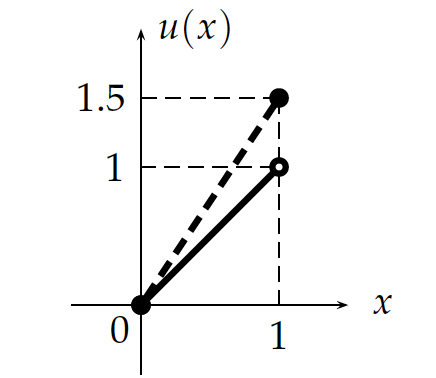
\includegraphics[scale = 0.4]{Images/sol.png}
    \label{fig:3}
  \end{figure}
  \noindent
  This problem has no solution, because the slope of $u(x)$ is 1 and
  at the boundary we have $u(1) = 1.5$. This means, we cannot find a
  solution that satisfies this Dirichlet Problem. This can be seen
  from the compatibility condition defined by
  (\ref{eq:13})-(\ref{eq:14}), as
  \begin{eqnarray}
    \lvert \varphi(1) - \varphi(0) \rvert = 1.5 \ge L(0,1) =
    \int_{0}^{1} 1 ds = 1
  \end{eqnarray}
  which does not satisfy the Compatibility condition (\ref{eq:14}).
\end{example}

\section{Comparison Theorem}
In this last section of the chapter, we study the uniqueness of the
solution to the Hamilton Jacobi Equation. We start with the classical
comparison principle to illustrate how uniqueness can be proved for
classical solutions. We then try to extend it to the viscosity setting
to study the uniqueness of the viscosity solution. Ishii\cite{ishii} in his work
presented and proved a comparison principle. Refer\cite{yong} for a detailed
version for the proof of the comparison theorem.

\subsection{Classical Comparison Theorem}
The classical version of the comparison theorem, involves assuming two
distinct solutions $u_1$ and $u_2$ solving the PDE, eventually showing
that they are equal. This is done by showing that,
\begin{equation}
  u_1 \le u_2, \quad u_2 \le u_1 \qquad in \;\;\; \bar{\Omega}
\end{equation}

\noindent
Refer \cite{yong} to see how this is done. The procedure followed here does not work for proving uniqueness for non-differentiable
solutions like $u(x) = \lvert x \rvert$, as the classical derivatives
are no longer defined at points of non-differentiability. To define
this in the viscosity setting, we have our new comparison theorem, by Ishii\cite{ishii}.

\subsection{Comparison Theorem}
In this section we state the formal statement of the comparison
theorem and see how that is used to conclude the uniqueness of the
viscosity solution.\\

\noindent
Before we state the theorem, we give the definition of modulus and a
couple of Hypothesis on the Hamiltonian $H$. Consider the following
HJE, with an Eikonal type Hamiltonian.
\begin{equation}
  H(x,Du(x)) = 0
\end{equation}

\begin{definition}
  \textbf{Modulus}: A function $m:[0,\infty[ \to [0,\infty[$ is called
  a modulus if its continuous and non-decreasing and satisfies $m(0) =
  0$
\end{definition}

\noindent
The two Hypothesis (H1) and (H2) on the Hamiltonian are stated below.
\begin{enumerate}
\item
  (H1) There is a modulus $m$ such that
  \begin{equation}
    \lvert H(x,p) - H(y,p)\rvert \le m (\lvert x-y \rvert (1+\lvert p \rvert))
  \end{equation}
  for $x,y \in \Omega$ and $p \in \mathbb{R}^n$
\item
  (H2) The function $p \to H(x,p)$ is convex on $\mathbb{R}^n$ for
  each $x \in \Omega$.

\end{enumerate}

\begin{theorem}
  \textbf{Comparison Theorem}\\

  \noindent
  Let $\Omega$ be a bounded open subset of $\mathbb{R}^n$. Assume that
  (H1) and (H2) holds. Let $\bar{u}$ and $\underset{\bar{}}{u} \in
  C^0$, respectively be viscosity super- and sub- solutions with
  \begin{equation}
    \underset{\bar{}}{u} \le \bar{u} \quad \text{on} \;\; \partial \Omega
  \end{equation}

  \noindent
  Also assume that\\

  (H3) $\exists$ a function $\varphi \in C^1(\Omega) \cap
  C^0(\bar{\Omega})$ such that, $\varphi \le \underset{\bar{}}{u}$ in
  $\bar{\Omega}$ and
  \begin{equation}
    \sup_{x\in \omega} H(x,D\varphi(x)) < 0 \qquad \forall \omega
    \subset \subset \Omega
  \end{equation}

  \noindent
  then $\underset{\bar{}}{u} \le \bar{u}$ in $\Omega$
\end{theorem}

\noindent
With this, we have the uniqueness result,
\begin{theorem}
  Let $u,v$ be two viscosity solutions of the Eikonal type HJE, such
  that $u = v \;\;\text{on} \;\;\partial \Omega$. Then $u = v$. Thus,
  the BVP,
  \begin{eqnarray}
    H(x,Du(x)) &=& 0 \qquad \text{in} \;\; \Omega\\
    u(x) &=& \varphi(x) \qquad \text{on} \;\; \partial \Omega
  \end{eqnarray}
  has atmost one viscosity solution.\\

  \noindent
  \textbf{Proof:} The proof is a direct consequence of the comparison
  theorem. As $u$ and $v$ are both viscosity sub- and super-solutions,
  by the comparison principle, $u \le v$ and $v \le u$ on $\Omega$. This implies
  $v = u$ on $\Omega$.
\end{theorem}
